\section{Git Object Model}

In this section, we will show the 
specification of the git object model, using as
basis two manuals, \cite{gitComm} and \cite{progit}. \par
Only the key parts of the model will be presented. \par

\subsection{Identification of Objects}

All objects are identified by a sha defined by their contents. \par
"All the information needed to represent the history
of a project is stored in files referenced by a 
40-digit {\bf "object name"}..." (page 7) \par
We don't need to specify this, as Alloy already can uniquely
identify atoms, so we can reutilize that functionality. \par


\subsection{The four types of Objects}

The objects are defined as in \cite{gitComm} (page 7) wich says: 
"...and there are four different types of objects: blob,
tree, commit, and tag."
Also: "A blob is used to store file data - it is generally a file" 
\cite{gitComm} (page 8). \par
For trees: "A tree is basically like a directory 
- {\bf it references a bunch
of other trees and/or blobs}..." (page 8) \par 

\begin{lstlisting}
abstract sig Object {
	objects : set State
}

sig Blob extends Object {}

sig Tree extends Object {
	contains : Name -> lone (Tree+Blob)
}
\end{lstlisting}

The tag will be discarded, as it doesn't affect the main operations
of git. \par 

Now for the commit:  
"As you can see,a commit is defined by : 
parent(s):{\bf The SHA1 name of some number of commits which
represent the immediately previous step(s) in the 
history of the project}..."
"...merge commits may have more than one. A commit with no 
parents is called a root commit, and represents the 
initial revision of a project. {\bf Each project must have at
least one root. A project can also have multiple roots,
though that isn't common (or necessarily a good idea)}". 
\cite{gitComm} (page12) 
A commit also points to a certain tree that represents the state of the
repository at a given state. \par

\begin{lstlisting}
sig Commit extends Object {
	points : Tree,
	parent : set Commit,
}
\end{lstlisting}

\section{Branches in Git}
One of the advantages of git compared to others VCS is the operation
of creating a new branch. While in others VCS, a copy of the hole project is
done each time we create new branch, in git, only a new pointer is created, as
said in the next quotations:
"A branch in Git is {\bf simply a 
lightweight movable pointer to one of these commits}." \cite{progit} (pag 39) \par
"The special pointer called {\bf Header 
points to the branch we are working on}". \cite{progit} (pag 40) \par

\begin{lstlisting}
sig Branch {
	marks : Commit one -> State
	branches : set State,
	head : set State
}
\end{lstlisting}

\section{Specification of files}

In order to model Git, we need the notion of a file. In our view a file should have
a path associated and a content. The path (along with it's parents)
will uniquely determine the full name of a file
(e.g. /x/y/example.txt), the content will be just a Blob.

\begin{lstlisting}
	sig File {
		path : Path,
		blob : Blob
	}

	sig Path {
		pathparent : lone Path,
		name : Name
	}
\end{lstlisting}

\begin{figure}[h!] 
	\caption{A typical example of a file, where is name is /Name1/Name0 }
	\centering
	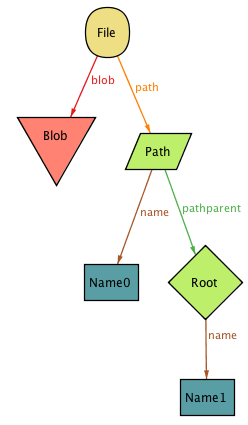
\includegraphics[scale=0.65]{images/image1.png}
\end{figure}
\pagebreak


\section{Index in Git}

The definition of Index:
"...staging area between your working directory and your
repository. You can use the index to {\bf build up a set of 
changes that you want to commit together}. When you create
a commit, {\bf what is committed is what is currently in the
index, not what is in your working directory.}"
\cite{gitComm} (page 17). \par

Also : ``The index {\bf contains all the information necessary to generate a single
(uniquely determined) tree object}'' \cite{gitComm} (pag 121). \par

Thus, what is in the index for a given state, is just a set of files.

\begin{lstlisting}
	sig File {
		path : Path,
		blob : Blob,
		index : set State
	}

\end{lstlisting}

\begin{figure}[h!] 
	\caption{A typical example of a file (file1) that is in the index}
	\centering
	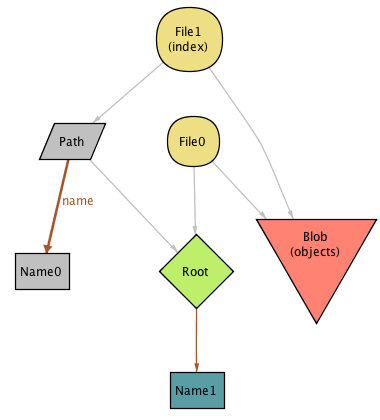
\includegraphics[scale=0.65]{images/image2.png}
\end{figure}
\pagebreak

